%% ===================================================================
%% paper.tex -- the complete research paper (Stage 14).
%% A copy of main.tex (the clean template) with the project title and the
%% author block of phase4_results.tex. Chapters live in sections/, copied
%% result tables in tables/, copied result figures in fig/ (both refreshed
%% with scripts/sync_paper_assets.sh; never edit the numbers by hand).
%% Based on bare_conf.tex V1.3 by Michael Shell (IEEEtran.cls)
%% Compile: see paper/BUILD.md (pdflatex -> biber -> pdflatex -> pdflatex).
%% ===================================================================

\documentclass[conference]{IEEEtran}
\usepackage{graphicx}
\usepackage{booktabs}
\usepackage{array}
\usepackage{amsmath}
\usepackage{amssymb}
\usepackage{microtype}
\usepackage{adjustbox}
\usepackage{etoolbox}
\usepackage{tikz}
\usetikzlibrary{positioning, arrows.meta, fit, calc}
\usepackage{url}
\usepackage[hidelinks]{hyperref}
\usepackage[backend=biber, style=ieee]{biblatex}

\addbibresource{ref.bib}

\graphicspath{ {fig/} }

% ---- ragged-right paragraph column for text-heavy tables: L{width} ----
\newcolumntype{L}[1]{>{\raggedright\arraybackslash}p{#1}}

% ---- float placement: lets large full-width tables place well ----
\setcounter{dbltopnumber}{4}
\renewcommand{\dbltopfraction}{0.99}
\renewcommand{\dblfloatpagefraction}{0.5}
\renewcommand{\topfraction}{0.95}
\renewcommand{\textfraction}{0.05}
\renewcommand{\floatpagefraction}{0.75}

% ---- copied result tables ------------------------------------------
% \PaperTable[layout]{file}{caption}
% Inputs tables/final_<file>.tex exactly as copied (every number and cell is
% untouched). Only the caption text is replaced (the source captions use
% internal stage names), and an optional layout code may change the float
% width or the font size for this paper.
\newcommand{\PaperTable}[3][]{%
  \begingroup
  \let\paperorigcaption\caption
  \renewcommand{\caption}[1]{\paperorigcaption{#3}}%
  #1%
  \input{tables/final_#2.tex}%
  \endgroup}
% layouts (layout changes only, never the content of a table):
%   \ColumnLayout  a table* of the source placed in one column
%   \WideLayout    a single-column table of the source placed across both columns
%   \SmallWide     a smaller font
% Every tabular that is wider than its float is scaled down to fit (adjustbox).
\newcommand{\ColumnLayout}{%
  \renewenvironment{table*}[1][t]{\begin{table}[##1]}{\end{table}}%
  \let\footnotesize\scriptsize}
\newcommand{\WideLayout}{%
  \renewenvironment{table}[1][t]{\begin{table*}[##1]}{\end{table*}}%
  \let\footnotesize\scriptsize}
\newcommand{\SmallWide}{\let\footnotesize\scriptsize}
\BeforeBeginEnvironment{tabular}{\begin{adjustbox}{max width=\linewidth}}
\AfterEndEnvironment{tabular}{\end{adjustbox}}

\begin{document}

\title{Resolution-Preserving Weakly Supervised\\ Recognition of Rice Leaf Diseases}

\author{\IEEEauthorblockN{Ahsan Baig, Harris Tabassum, and Muhammad Umer}
\IEEEauthorblockA{23L-0515, 23L-0551, 23L-0845\\
FAST School of Computing\\
National University of Computer and Emerging Sciences (FAST-NUCES)\\
Lahore, Pakistan\\
Email: \{l230515, l230551, l230845\}@lhr.nu.edu.pk}}

\maketitle

\begin{abstract}
Rice leaf photos are taken at high resolution, but most recognition systems shrink them to a few
hundred pixels, and many reports do not say how the data were split.
We study a resolution-preserving alternative that needs only photo-level labels. Each photo is
brought to a common leaf scale and cut into 224-pixel tiles. A frozen DINOv3 encoder describes every tile once,
and a small gated-attention head, trained from the photo label alone, combines the descriptions and
produces a heat map. We compare it with four fine-tuned whole-image models, probes, simpler pooling rules and
ablations. The protocol groups near-duplicates and capture sessions, reports macro-F1 and balanced accuracy with
spread and bootstrap ranges, and adds a zero-shot test on field photos (Paddy Doctor).
On the session-blocked split the head reaches 77.9\,\% test macro-F1. It is clearly above two of the four
whole-image models at 224 px and above both whole-photo controls, and not clearly different from ConvNeXt-T at
448 px, which has the higher mean. A committee of the two is clearly better than either.
Zero-shot transfer to field photos is not shown: all methods score low.
Removing the most-attended tiles hurts far more than removing random tiles.
Augmenting before splitting raises the score by 11.5 to 17.2 points, which shows how much the split order matters.
The price is about 80 encoder passes per photo. Negative results are reported as they are.

\end{abstract}

\begin{IEEEkeywords}
Rice leaf disease, multiple instance learning, attention pooling,
self-supervised features, grouped evaluation, zero-shot transfer
\end{IEEEkeywords}

\IEEEpeerreviewmaketitle

\section{Introduction}
\label{sec:intro}

Rice (\textit{Oryza sativa}) feeds about half of the world's population and is grown on more than 160 million
hectares \cite{faostat2024}. Pathogens and pests cause a mean yield loss of roughly 30\,\% in rice, the highest among
the five major food crops \cite{savary2019}. Rice is Pakistan's second most important cereal after wheat
\cite{gopk2024}. A foliar disease can be controlled only in a short window, and there are too few extension officers
to inspect every field, so an image-based diagnosis that works on photos a farmer can take would remove a real
bottleneck.

Automated recognition has moved from hand-made features to fine-tuned convolutional networks, transformers and generative
augmentation (Section~\ref{sec:related}), but one formulation has stayed the same: one label is predicted from one strongly
downsampled view of the photo. That is a poor match to the task. A lesion can fill well under 1\,\% of the frame, so a
photo of $1881\times1881$ pixels \cite{do2019} shrunk to $224\times224$ keeps about 1 pixel in 70, and the pale centre or
halo that separates brown spot from leaf blast is averaged away.

Three gaps follow from the literature reviewed in Section~\ref{sec:related}.
(i) Resolution is fixed early and never varied, although region aggregation is standard for gigapixel pathology images
\cite{ilse2018, lu2021clam}. (ii) Background suppression is either hand-made or needs annotation; a learned method that
uses photo-level labels only has not been evaluated for rice. (iii) Reporting practice makes numbers hard to compare:
the order of splitting and augmenting is often unstated, accuracy on imbalanced data is the usual metric, and
cross-dataset tests are rare. Testing problems of this kind are common in the field \cite{xu2024}, and a model above
90\,\% on several benchmarks has been reported at 58.15\,\% on an unseen rice set \cite{thakur2023}.

We therefore treat resolution as a variable and the protocol as part of the contribution. The method keeps lesion-scale
detail by cutting each photo into high-detail tiles at a common leaf scale, describing every tile with a frozen
self-supervised encoder, and letting a small attention head learn from the photo label which tiles matter. This is
multiple instance learning (MIL): a photo is a labelled bag of unlabelled tiles. The contributions are:
\begin{itemize}
\item a tile-and-attention pipeline for rice leaf disease that trains only about a quarter of a million parameters,
and its heat maps (Section~\ref{sec:method});
\item a protocol that groups near-duplicates and capture sessions, fixes the split before augmentation, reports
spread and two bootstrap ranges, and states a rule for ``A beats B'' (Section~\ref{sec:setup});
\item controlled comparisons on resolution, pooling, Otsu preprocessing and encoders, a zero-shot test on field photos,
a deletion test of the heat maps, a cost measurement, and a partition-order experiment on how much a faulty split
raises the score (Section~\ref{sec:results}).
\end{itemize}
Five hypotheses, fixed before the experiments, structure the study:
\textbf{H1}, tiles beat whole-photo input with the same encoder;
\textbf{H2}, the learned attention is at least as good as mean pooling, max pooling and Otsu preprocessing;
\textbf{H3}, frozen features hold up on unseen field photos;
\textbf{H4}, the heat map points at real symptoms;
\textbf{H5}, the cost is reasonable and can be reduced.
Section~\ref{sec:related} reviews related work, Section~\ref{sec:method} describes the method,
Section~\ref{sec:setup} the data and protocol, Section~\ref{sec:results} the results, and
Sections~\ref{sec:discussion}--\ref{sec:conclusion} discuss them, state the limits and conclude.

% Adapted from the frozen Phase 2 submission.
\section{Literature Review}
\label{sec:lit}
% ===================================================================

\subsection{Review Scope and Methodology}

Candidate studies were located through Google Scholar, IEEE Xplore, ScienceDirect,
SpringerLink and PubMed Central using combinations of the terms \emph{rice leaf
disease}, \emph{plant disease classification}, \emph{multiple instance
learning}, \emph{patch-based}, \emph{foundation model}, \emph{data augmentation},
\emph{disease severity} and \emph{edge deployment}. Studies were included if they
reported a quantitative evaluation on rice or on closely related foliar disease
imagery, or if they introduced a methodological component that the proposed
pipeline depends upon. Twenty-six studies are characterised in the survey tables;
of these, twenty-one were published between 2020 and 2026, with the remaining
five retained because they are the methodological origin of a technique the
project builds on. A small number of additional works are cited in the discussion
purely as methodological anchors and are not tabulated: the multiple instance
formulation \cite{dietterich1997}, attention-based instance aggregation
\cite{ilse2018}, its weakly supervised application in computational pathology
\cite{lu2021clam}, Otsu's thresholding operator \cite{otsu1979}, the paired
image-to-image translation model used for generative augmentation in the rice
literature \cite{isola2017}, and the residual and transformer backbones that
recur as baselines \cite{he2016, dosovitskiy2021}.

Tables~\ref{tab:survey1} and~\ref{tab:survey2} summarise each study by reference,
year, method, dataset, evaluation metrics, reported performance and key
limitations. Where a study reports qualitative results or metrics that are not
comparable across the table, the performance column describes the reported
outcome rather than quoting a single figure.
\clearpage



\subsection{Critical Discussion by Methodological Group}

\subsubsection{Classical image processing and handcrafted features}

The earliest rice-specific systems operated on explicitly engineered
representations. Orillo \textit{et al.} segmented lesions in MATLAB and
classified colour and texture descriptors with a back-propagation network,
reporting perfect accuracy on 134 images \cite{orillo2014}; Pugoy and Mariano
combined histogram intersection with $k$-means clustering to isolate outlier
regions \cite{pugoy2011}; Azim \textit{et al.} used a saturation threshold to
remove background and a hue threshold to isolate lesions before applying XGBoost
\cite{azim2021}; and Sethy \textit{et al.} occupy an intermediate position,
extracting CNN features but classifying them with an SVM \cite{sethy2020}. Two
observations matter for this project. First, the reported accuracies are
uninformative as generalisation estimates: a 100\,\% score on 134 images
\cite{orillo2014} and comparable figures on the 120-image UCI subset
\cite{azim2021} reflect dataset size far more than method quality. Second, and
more usefully, this group establishes the \emph{lineage} of the thresholding
operations that persist in modern pipelines. When a recent deep pipeline applies
Otsu thresholding as a preprocessing stage \cite{ali2026}, it is inheriting a
design decision from this era, with the same underlying assumption of a clean
bimodal separation between leaf and background. That assumption is testable, and
the evidence within the literature is mixed at best: one study using the same
rice dataset describes its backgrounds as essentially uniform and therefore not
requiring background subtraction \cite{tejaswini2022}, while the same operator
applied to raw images of that dataset has been reported to leave classifier
accuracy largely unchanged \cite{ali2026}.

\subsubsection{CNN transfer learning}

This is by far the largest group and it is also the most saturated. Following
Mohanty \textit{et al.} \cite{mohanty2016}, rice-specific studies have applied
essentially every mainstream ImageNet backbone to essentially the same handful of
public datasets \cite{lu2017, chen2020, ghosal2020, tejaswini2022}. The pattern
of reported results is more revealing than any individual number. On the same
Kaggle rice dataset, published accuracies span 58.15\,\% \cite{thakur2023},
74--78\,\% \cite{tejaswini2022, ali2026} and 86.98\,\% \cite{ali2026}, a spread
of nearly thirty points across differing protocols. Partitioning, preprocessing,
augmentation and metric definitions may contribute to these differences; the
reported scores do not isolate architecture. This motivates the internally
consistent baseline comparisons in the present study. The group also shares two structural
limitations. Input resolution is fixed early and never ablated, and evaluation is
almost exclusively in-domain and accuracy-based. Ghosal and Sarkar's report of
92.46\,\% training against 81\,\% test accuracy \cite{ghosal2020} is a useful
illustration of how much information a single accuracy figure conceals.

\subsubsection{Transformers and hybrid architectures}

Recent work substitutes or supplements the convolutional backbone with
self-attention \cite{alfalluji2025, vitresnet2025, globallocal2026}. The trend is
towards two-stream designs in which a transformer branch captures global context
and a convolutional branch captures local texture, fused by a learned attention
mechanism \cite{globallocal2026}. Two of these studies provide additional evaluation detail: Ramesh \textit{et al.}
report precision, recall, F1 and AUC rather than accuracy alone
\cite{vitresnet2025}, and the two-stream study includes both cross-validation and
cross-dataset testing \cite{globallocal2026}. Nevertheless, the group is subject
to diminishing returns. Accuracies of 100\,\% and 99.72\,\% on a three-class rice
task \cite{alfalluji2025} indicate that the benchmark, not the method, is the
limiting factor; notably, the same study's accuracy falls to 90.69\,\% on a
five-class task, a drop that is reported but not diagnosed. Critically, every
model in this group still performs a single forward pass over one downsampled
view of the leaf. A hierarchical transformer attends across patches \emph{within}
a $224\times224$ input, which is a different operation from attending across
regions of the original $1881\times1881$ capture; the information discarded by
the resize is not recoverable by attention applied afterwards. This distinction
is central to the gap this project targets.

\subsubsection{Generative data augmentation}

Two sub-lines exist. Adversarial approaches dominate the rice literature: the
pipeline most directly relevant to this project pairs a Pix2Pix generator with
Otsu preprocessing and an InceptionDenseNet classifier \cite{ali2026}, and more
recent work improves generator fidelity through frequency-domain and
dual-discriminator designs \cite{fhwd2025}. Diffusion-based augmentation is the
emerging alternative and has been reported to produce more realistic and more
diverse plant disease imagery than comparable GANs \cite{muhammad2023}. Three
experimental considerations follow. First, fidelity is not the objective: FID measures how
convincing an image looks, not whether adding it to the training set improves
generalisation, and the causal link between the two is assumed far more often than
it is demonstrated. Second, the rice literature contains a clear negative result
worth taking seriously --- adversarial augmentation applied on its own has been
reported to \emph{reduce} classifier accuracy relative to the raw data, with
improvement appearing only when combined with a preprocessing stage
\cite{ali2026}. Third, paired image-to-image generation such as Pix2Pix \cite{isola2017}
requires an explicit conditioning representation and paired training data. This
adds an experimental factor alongside the classifier and preprocessing. The
present study therefore uses conventional augmentation and focuses on spatial
representation and aggregation; it does not test whether synthetic augmentation
would improve this protocol.

\subsubsection{Segmentation-based preprocessing and severity quantification}

A different response to background clutter replaces
thresholding with a learned segmentation network. RCAMNet performs multi-class
segmentation with U-Net, DeepLabv3 or Detectron2 and then applies dual-path
attention for joint classification and severity staging \cite{sudhesh2025}, while
a UAV study reaches 97.20\,\% mIoU using U-Net with a ResNet-101 encoder on
multispectral imagery scored against the IRRI Standard Evaluation System
\cite{logavitool2025}. These results confirm that lesion-level supervision, when
available, is highly effective. The binding constraint is annotation. Both studies
depend on purpose-built datasets with expert pixel-level labels, and the public
rice datasets in general use provide no masks; the recently released
\textit{RiceSeg-5932} mask collection \cite{riceseg2025} addresses this for a
different rice image set but not for the datasets used here. There is also a
subtler point: segmentation removes background but does not address resolution,
since the segmented image is still resized before classification. A method that
requires no masks and preserves resolution is therefore preferable on both counts,
and this reasoning is why segmentation is treated in this project as a comparison
point rather than as the proposed solution.

\subsubsection{Patch-level, lesion-level and weakly supervised learning}

This group contains the nearest precedents for the proposed method and is, at the
same time, the thinnest group in the plant disease literature. DeChant
\textit{et al.} tile field images of maize, classify each region with a CNN,
assemble the per-region outputs into heat maps, and classify the whole image from
those maps, reaching 96.7\,\% on held-out data \cite{dechant2017}. Barbedo shows
that classifying individually cropped lesions substantially outperforms
whole-leaf classification across fourteen species \cite{barbedo2019}. Bollis
\textit{et al.} use activation maps to propose regions and then apply multiple
instance learning over them for citrus pest classification \cite{bollis2020}.
The formulation these works approach is multiple instance learning
\cite{dietterich1997}, in which a labelled \emph{bag} of unlabelled
\emph{instances} is classified as a whole; in its modern form, a learned
attention function assigns each instance a weight and the bag representation is
their weighted mean \cite{ilse2018}, a design that underpins clinical-grade
weakly supervised classification of gigapixel pathology slides
\cite{lu2021clam}. The structural correspondence to leaf imagery is close: a
high-resolution image, a diagnostic region occupying a small fraction of it, and
a label available only at whole-image level. What is missing is the combination.
DeChant \textit{et al.} require manual lesion marking to train the region
classifier and use a fixed, non-learned aggregation \cite{dechant2017}; Barbedo
requires lesions to be cropped by hand \cite{barbedo2019}; Bollis \textit{et al.}
use a two-stage saliency-then-MIL design on a pest task \cite{bollis2020}. To the
best of our knowledge, no published work applies end-to-end attention-based
instance aggregation over high-detail tiles, trained from image-level
labels alone, to rice leaf disease recognition. This is the methodological centre
of the gap identified in Section~\ref{sec:gap}.

\subsubsection{Foundation models and frozen self-supervised features}

Self-supervised vision transformers trained on web-scale unlabelled imagery
\cite{oquab2024} have recently been evaluated in agriculture with results that
are directly relevant here. Foundation features have been assessed in agriculture
under linear probing, full fine-tuning and low-rank adaptation, with the frozen
linear probe remaining competitive at a small fraction of the training cost and
foundation features outperforming other self-supervised alternatives when
distilled into a mobile backbone \cite{dinoagri2025}. More pointedly, frozen
self-supervised features have been shown to substantially reduce the
laboratory-to-field degradation that afflicts supervised backbones
\cite{nguyen2026}, and contrastive self-supervised pretraining under an explicit
leakage-controlled protocol improves robustness under domain shift
\cite{plantclr2026}. Two properties make this group attractive as a component
rather than a contribution. Because a frozen encoder is never trained on the
target data, it cannot memorise dataset-specific background cues, which is
exactly the failure mode that motivates background removal in the first place.
And because embeddings can be computed once and cached, the cost of aggregating
many regions per image becomes tractable, which is what makes a tile-based
formulation feasible under student-level compute. The gap is that all of these
studies probe features from whole downsampled images; none evaluates frozen
features as region descriptors under a weakly supervised aggregator, and none
targets rice.

\subsubsection{Datasets, evaluation protocol and generalisation}

This group supplies the evidence for the protocol gap. Xu \textit{et al.}
provide a taxonomy of plant disease datasets and argue that the apparent success
of deep learning in this field is partly illusory, identifying random splitting
as a direct cause of overestimated test performance because near-duplicate views
of one physical observation can be distributed across training and test
partitions, and observing that splitting and annotation strategy are scarcely
discussed in applied papers \cite{xu2024}. This is a field-wide reporting issue
rather than a fault of any individual study: where the ordering of augmentation
and partitioning, or the partition on which a confusion matrix was computed, is
not stated, the reader simply cannot determine what a reported figure measures.
The consequences are visible empirically. A model exceeding 90\,\% on four
benchmarks reaches 58.15\,\% on an unseen rice dataset \cite{thakur2023}, and
the laboratory-to-field drop documented for frozen-feature studies
\cite{nguyen2026, plantclr2026} is larger than the margins by which competing
architectures are separated. On the resource side, the group also supplies the
remedy. Paddy Doctor offers 16{,}225 expert-annotated field images across 13
classes with published transfer-learning baselines and an F1-based reporting
convention \cite{petchiammal2023}, and PlantDoc demonstrates the value of
deliberately in-the-wild data for breaking laboratory shortcuts
\cite{singh2020}. The availability of a large, independently collected field
dataset whose class vocabulary overlaps the primary dataset is what makes the
zero-shot cross-dataset evaluation in objective~6 practical rather than
aspirational.

\subsubsection{Lightweight models and edge deployment}

The final group addresses whether a model can run where it is needed.
MobileNet-V4 has been benchmarked against earlier mobile backbones across GPU,
CPU and Raspberry Pi 5, reporting 97.84\,\% accuracy at 88.91\,ms per inference
on the Pi \cite{edge2026}, and structured pruning combined with channel-wise
feature distillation compresses a YOLOv11 variant to 1.9\,MB while retaining
97.4\,\% mAP@50 \cite{liu2025}. These studies are notable for measuring latency
on real hardware rather than asserting deployability, a standard that much of the
rice literature does not meet --- claims that a 98\,MB classifier is suitable for
IoT or edge use are common but are rarely accompanied by an on-device
measurement. The limitation is that this group optimises for in-domain accuracy
under compression and does not test whether the compressed model retains
generalisation. For this project the group functions as a cost benchmark: any
region-based pipeline must be assessed for computational overhead against these
figures, which is the purpose of objective~7.

\subsection{Synthesis: Cross-Cutting Limitations}

Reading across the nine groups, four limitations recur with enough consistency to
be treated as properties of the field rather than of individual papers. Input
resolution is treated as a fixed preprocessing constant and is never ablated,
despite the two-order-of-magnitude information loss it entails on
high-resolution captures. Background suppression is addressed at opposite
extremes of the supervision spectrum --- hand-tuned global operators on one side
\cite{ali2026, azim2021} and densely annotated segmentation networks on the other
\cite{sudhesh2025, logavitool2025} --- with no annotation-free learned option
evaluated in between. Overall accuracy on a randomly partitioned, strongly
imbalanced dataset remains the dominant metric, so a model that never predicts a
rare but agronomically important class pays almost no measured penalty, and
repeated runs with reported variance are uncommon. Finally, cross-dataset
evaluation is rare enough that the field-readiness claims made in the motivation
sections of these papers are, in most cases, untested by their own experiments.

It is worth being explicit that the four are connected rather than independent.
Aggressive downsampling removes lesion-scale evidence, which leaves the
classifier more reliant on whatever global cues are available, including
background and acquisition artefacts; that reliance is invisible under in-domain
accuracy on a randomly split single dataset, and surfaces only under
cross-dataset evaluation, where it appears as the large degradations reported in
\cite{thakur2023, nguyen2026}. A method that preserves resolution and learns
region relevance therefore addresses the measurement problem and the modelling
problem through the same mechanism, provided the evaluation is designed to detect
the difference.

\subsection{Research Gap}
\label{sec:gap}

Three gaps follow directly from the synthesis above.

\begin{itemize}
\item \textbf{Resolution gap.} Rice disease recognition pipelines almost
universally downsample high-resolution captures to between 128 and 256 pixels
before classification, discarding the fine textural evidence that distinguishes
early-stage and visually similar lesions. No study in the reviewed literature
treats input resolution as an experimental variable, and none evaluates
resolution-preserving region aggregation as an alternative, although the
technique is standard in gigapixel medical imaging \cite{ilse2018, lu2021clam}.

\item \textbf{Supervision gap.} Suppression of diagnostically irrelevant image
content is handled either by hand-engineered global operators that assume a
bimodal leaf--background separation \cite{ali2026, azim2021, otsu1979}, or by
segmentation networks that require pixel-level masks unavailable for the public
rice datasets \cite{sudhesh2025, logavitool2025}. An annotation-free mechanism
that \emph{learns} which regions are informative from image-level labels alone
has been demonstrated in maize and citrus in partial forms
\cite{dechant2017, barbedo2019, bollis2020} but has not been evaluated for rice
in an end-to-end attention-based formulation.

\item \textbf{Protocol and generalisation gap.} Reported performance in this
field is difficult to interpret and difficult to compare, because partitioning
strategy and the ordering of augmentation relative to partitioning are often
unstated \cite{xu2024}, class-balanced metrics and run-to-run variance are often
unreported, and zero-shot evaluation on an independently collected dataset is
rare. Consequently the generalisation claims that motivate the work are largely
unsupported by the experiments presented, as the observed collapse from above
90\,\% to 58.15\,\% on an unseen rice dataset illustrates \cite{thakur2023}.
\end{itemize}

\subsection{Problem Statement}

Given high-resolution rice leaf images annotated only with an image-level
disease label, the problem is to classify the disease while (i) preserving
lesion-scale spatial detail rather than discarding it through whole-image
downsampling, (ii) suppressing diagnostically irrelevant regions through a
learned mechanism that requires no pixel-level supervision, and (iii) reporting
the result under an evaluation protocol that fixes partitioning before any
augmentation, reports class-balanced metrics with variance across repeated runs,
and, in the broader planned study, measures zero-shot transfer to an
independently collected field dataset with overlapping disease classes. The
present submission evaluates the in-domain component; external generalisation
remains untested. The proposed approach treats each leaf image as a
collection of high-detail regions at a common leaf scale and learns, from image-level labels
alone, both a class prediction and an attention distribution over regions
showing the model's learned weighting of the regions. These visual weights
are descriptive; causal faithfulness requires the separately planned tests.

\medskip


\section{Method}
\label{sec:method}

This section describes the pipeline in Fig.~\ref{fig:pipeline}: tile the photo at a common leaf scale, describe each
tile once with a frozen encoder, and combine the descriptions with a small trained attention head.

\begin{figure}[t]
\centering
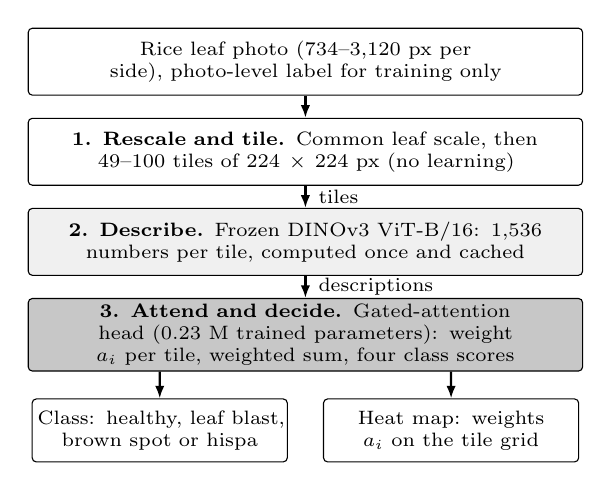
\begin{tikzpicture}[
  font=\scriptsize,
  box/.style={draw, rounded corners=1.5pt, align=center, minimum height=0.85cm, text width=6.9cm, inner sep=2pt},
  frozen/.style={box, fill=black!6},
  trained/.style={box, fill=black!22},
  outbox/.style={draw, rounded corners=1.5pt, align=center, minimum height=0.8cm, text width=3.1cm, inner sep=2pt},
  arrow/.style={-{Latex[length=1.6mm]}, thick}]
  \node[box] (photo) {Rice leaf photo (734--3{,}120 px per side), photo-level label for training only};
  \node[box, below=0.28cm of photo] (tile) {\textbf{1. Rescale and tile.} Common leaf scale, then 49--100 tiles of $224\times224$ px (no learning)};
  \node[frozen, below=0.28cm of tile] (enc) {\textbf{2. Describe.} Frozen DINOv3 ViT-B/16: 1{,}536 numbers per tile, computed once and cached};
  \node[trained, below=0.28cm of enc] (att) {\textbf{3. Attend and decide.} Gated-attention head ($0.23$ M trained parameters): weight $a_i$ per tile, weighted sum, four class scores};
  \node[outbox, below=0.34cm of att, xshift=-1.85cm] (lab) {Class: healthy, leaf blast, brown spot or hispa};
  \node[outbox, below=0.34cm of att, xshift=1.85cm] (map) {Heat map: weights $a_i$ on the tile grid};
  \draw[arrow] (photo) -- (tile);
  \draw[arrow] (tile) -- node[right, xshift=1pt] {tiles} (enc);
  \draw[arrow] (enc) -- node[right, xshift=1pt] {descriptions} (att);
  \draw[arrow] (att.south) ++(-1.85,0) -- (lab.north);
  \draw[arrow] (att.south) ++(1.85,0) -- (map.north);
\end{tikzpicture}
\caption{The pipeline. White boxes: no learning; light grey: frozen encoder; dark grey: the only trained part.
Only the photo-level label is used for training.}
\label{fig:pipeline}
\end{figure}

\subsection{Common leaf scale and tiles}
A 224-pixel tile covers a different amount of leaf in photos of 734 and 3,120 pixels, so we first brought every photo to a
common leaf scale. The scale rule is described in Section~\ref{sec:setup}; it predicts the leaf width
$\hat w(s)=\exp(b+a\log s)$ in pixels from the shorter side $s$, with $a=0.776456$ and $b=-0.557512$, and rescales the photo
by $194.9/\hat w(s)$, where 194.9 px is the median measured leaf width (Section~\ref{sec:setup:data}). The rescaled shorter sides run from 1,488 to
2,056 px. For a side of length $L$ we cut $n=\lceil L/224\rceil$ square $224$-px tiles per axis, with starts evenly spaced
from $0$ to $L-224$ (integer pixel positions by floor division), so the tiles cover the whole photo, background
included. This gives 49--100 tiles per photo and 265{,}349 in all. We call the result ``high-detail tiles at a common
leaf scale''; tiles at the stored resolution (the \emph{native scale}) and tiles of Otsu-cleaned photos are ablations
(Section~\ref{sec:results}).

\subsection{Frozen description}
A frozen DINOv3 ViT-B/16 encoder \cite{simeoni2025dinov3} turned each tile into tokens: one class token, four register
tokens \cite{darcet2024registers} and the patch tokens. The descriptor of a tile is the 768-number class token $\mathbf c_i$
joined with the 768-number mean $\mathbf m_i$ of the patch tokens, which excludes the class and register tokens
($\mathbf h_i=[\mathbf c_i;\mathbf m_i]$, 1{,}536 numbers; descriptors using only $\mathbf c_i$ or only $\mathbf m_i$ are
ablations). Descriptions were computed once and cached for eight versions of each photo (the clean photo and augmented versions;
only the clean one is used for validation and test); the encoder (85.7 M parameters) is never updated, so it cannot memorise the photos.

\subsection{Gated-attention head}
For a bag of descriptors $\{\mathbf h_i\}$ a learned layer gives
$\mathbf g_i=\operatorname{Dropout}(\operatorname{ReLU}(W_p\mathbf h_i+\mathbf b_p))$. The gated attention of Ilse
\textit{et al.}\ \cite{ilse2018} scores and normalises the tiles and forms the photo representation $\mathbf z$:
\begin{align}
 e_i &= \mathbf v^{\top}\bigl[\tanh(V\mathbf g_i+\mathbf b_V)\odot\sigma(U\mathbf g_i+\mathbf b_U)\bigr],\\
 a_i &= \frac{\exp(e_i)}{\sum_j\exp(e_j)},\qquad
 \mathbf z=\sum_i a_i\mathbf g_i .
\end{align}
A linear layer maps $\mathbf z$ to four class scores. Only the projection, the attention parameters and this layer are
trained (0.23 M parameters). During training we dropped tiles at random with a tuned probability and always kept at
least one. The weights $a_i$ sum to one over the photo; painted on the tile footprints (overlaps averaged, scaled to
each photo's maximum), they form the heat map. They describe where the head looked and are not a segmentation. We call the full model Attention MIL.

\subsection{Variants}
Replacing the attention with the mean or the elementwise maximum of the $\mathbf g_i$ gave the pooling controls
(Mean pooling over tiles, Max pooling over tiles). Applying the head to one description of the whole photo, at 224 or
512 px, gave the whole-photo controls (Same head, whole photo); a bag of one tile has no attention to learn. The
Committee averages the class probabilities of ConvNeXt-T (448 px) and Attention MIL, and the Small model (16 tiles) keeps only the 16 tiles ranked
highest by a simple colour rule, to cut the number of encoder passes (Section~\ref{sec:results}).

\section{Experimental Setup}
\label{sec:setup}

This section describes the data, the two splits, the comparison models, the tuning and the rule used to compare methods.
The duplicate review, background audit, label check and heat-map ratings were done by disclosed AI model raters; one of
the two leaf-width measurers was also an AI model.

\subsection{Data}
\label{sec:setup:data}
The primary data are the labelled photos of the Rice Diseases Image Dataset \cite{do2019} (MIT licence; Kaggle release last updated 2019-11-15, downloaded on
2026-09-26): 3{,}355 photos of healthy leaves (1{,}488), leaf blast (779), brown spot (523) and hispa (565), with shorter
sides of 734--3{,}120 px (Fig.~\ref{fig:samples}). The download holds two more hispa photos than the published count (563). Three phone cameras
appear, and hispa photos all come from one of them.
A two-stage check (perceptual hash or embedding similarity, then a keypoint match) flagged near-duplicates, and two model
raters reviewed the candidates (Cohen's $\kappa$ \cite{cohen1960kappa} of 0.77; the 61 disagreements were adjudicated
and both original verdicts were kept). It confirmed 349 same-leaf pairs. Twenty-one photos that appear under
two different labels were excluded, which leaves 3{,}334 photos in 3{,}045 near-duplicate groups for all experiments.
A background audit of 240 photos (60 per class) found every background plain, and a label check of 80 photos
found one that looked like another class; no label was changed.

The leaf-scale rule rests on a pixel-scale audit. We measured leaf width on 30 photos spread over the size range (29 were
measurable). Width and shorter side correlated with Spearman $\rho=0.539$, above the pre-declared threshold of 0.5, so
photos are rescaled. The audit is borderline: leave-one-out correlations run from 0.488 to 0.613. The two measurers
agreed closely ($\rho=0.978$).

Paddy Doctor \cite{petchiammal2023} (full release from IEEE DataPort, DOI 10.21227/hz4v-af08; CC BY 4.0; downloaded on 2026-09-26) has 16{,}225 field photos of $1080\times1440$ px
in 13 classes. Its four classes shared with the primary data hold 8{,}086 photos once 78 byte-identical copies are
removed; none matches a primary photo. It was used only for zero-shot scoring, never for training, tuning or selection. A
224-px tile covers about three times more leaf on Paddy Doctor photos than on rescaled primary photos (median leaf width
194.9 against 64.5 px; the second value is a model-rater estimate from 30 photos of the nine classes we did not test).
We therefore scored three zoom levels: native, in which the photo is tiled as stored and which was fixed in advance as the
headline; midway ($\times1.73$); and matched ($\times3.0$).

\begin{figure}[t]
\centering
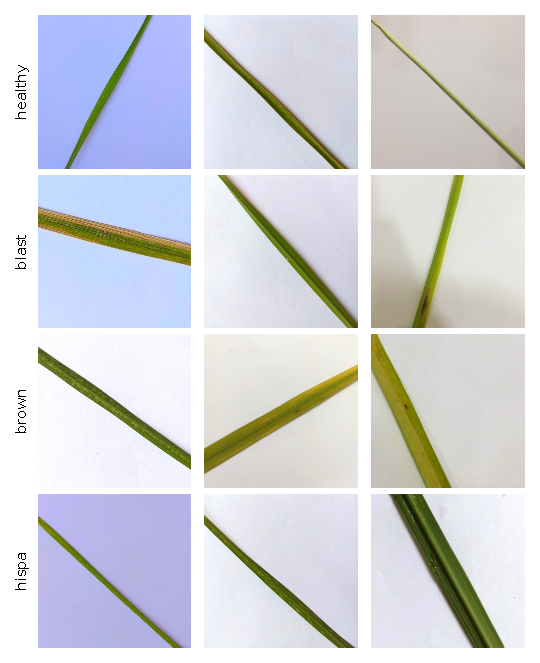
\includegraphics[width=0.6\columnwidth]{final_samples.pdf}
\caption{Example photos of the primary dataset: three per class (rows: healthy, leaf blast, brown spot, hispa).}
\label{fig:samples}
\end{figure}

\subsection{Splits}
\label{sec:setup:splits}
Each split was made once, before any model was trained on it, and is never regenerated; the locked split was made before any other processing. The \emph{locked split} is a stratified,
near-duplicate-grouped five-fold split (seed 2026). In each round one fold is the test set, and a stratified, grouped
$1/8$ of the rest is validation, giving about 70\,\%, 10\,\% and 20\,\% of the photos. Because photos were shot in
long sessions, it still lets a test photo have a training photo of the same camera a few seconds away (90.2\,\% of test
photos within 10 s). The \emph{session-blocked split} therefore keeps whole capture blocks (runs of photos of one camera
with no pause over 60 s; 74 blocks, the largest holding 287 photos) on one side: no test photo has a same-camera training photo within 60 s. It uses the same folds procedure
and the same validation rule. Block sizes make class shares uneven across rounds (worst deviation 26.5 points); they are
reported, not enforced. Test sets hold 616--738 photos. The session-blocked split was declared after the locked-split test
results were seen, and every method was then tuned again on its validation photos; it is the headline split, and the
locked split is the secondary one. Augmented copies stay in the role of their source photo and never reach validation or
test, which automated tests enforce.

\subsection{Comparison models}
Four ImageNet-pretrained models were fine-tuned on whole photos, padded to a square and resized:
InceptionV3 \cite{szegedy2016inception}, EfficientNetV2-S \cite{tan2021efficientnetv2}, ConvNeXt-T \cite{liu2022convnext}
and Swin-T \cite{liu2021swin}, at 224 px; at 128 px; at 224 px after Otsu background removal; and, for ConvNeXt-T, which
had the best validation score at 224 px, at 448 px. Linear probes at 224 and 512 px fit class-balanced
logistic regression on one frozen DINOv3 description of the whole photo. Six controls see no leaf shape: majority class, random by class
share, colour only, background only, file properties only and camera only; a seventh predicts the class of the nearest
training photo in time from the same camera.

\subsection{Training and selection}
\label{sec:setup:training}
All trained models used inverse-frequency class weights and cross-entropy with label smoothing 0.1
\cite{muller2019labelsmoothing}; we generate no images. Training photos were augmented with random resized crops, flips,
rotations and colour changes. Fine-tuning used AdamW \cite{loshchilov2019adamw} with weight decay 0.05, two warm-up epochs
and a cosine decay \cite{loshchilov2017sgdr}, mixed precision \cite{micikevicius2018mixed}, batches of 32, at most 40
epochs and patience 8 on validation macro-F1. For each architecture three learning rates ($3\times10^{-5}$, $10^{-4}$,
$3\times10^{-4}$) were tried in all five rounds, and the grid was extended by at most three further values when the best was
at an edge. Each aggregator head (attention, mean, max, and the whole-photo head) received 40 Optuna trials
\cite{akiba2019optuna} per study over learning rate, weight decay, projection width, dropout, tile dropout and descriptor,
in two studies with different learning-rate ranges, and kept the better; the probes searched six L2 strengths. Every
choice used the mean validation macro-F1 over the five rounds. Budgets match within a method family and differ across
families. Models were trained with PyTorch \cite{paszke2019pytorch}, timm \cite{wightman2019timm}, Transformers
\cite{wolf2020transformers} and scikit-learn \cite{pedregosa2011sklearn}, on an RTX 4060 (8\,GB) with a Ryzen 7 7700 and
16\,GB of RAM; some description caches were built on Kaggle T4 GPUs or a second PC (each cache on one machine). Every run
record keeps the configuration, code commit, split checksum, and per-photo predictions.

\subsection{Metrics and the comparison rule}
\label{sec:setup:metrics}
The main metric is macro-F1, the mean over the four classes of the F1 score, with balanced accuracy (the mean recall). We also
report per-class recall, confusion matrices (from which per-class precision follows; Table~\ref{tab:final_confusion}) and the expected calibration error (ECE, 15 equal-width bins
\cite{guo2017calibration}). Every table gives the mean $\pm$ SD over the five test rounds; there is one training seed per
round, so the SD measures variation over folds, not over seeds; the model trained in a round is its ``round-model''. Differences between two methods are computed on the
pooled test predictions (every photo once) and come with two 95\,\% percentile bootstrap ranges \cite{efron1993bootstrap}:
the \emph{photo range} resamples photos (2{,}000 class-stratified resamples) and the \emph{block range} resamples whole
capture blocks, and is wider when neighbouring photos look alike. ``A beats B'' requires the range of the difference to lie
above zero \emph{and} A to win at least four of the five rounds (a tied round is won by neither); we state the verdict
under both ranges, and otherwise write ``no clear difference''. Plain accuracy is kept in every run record. Each frozen configuration was evaluated on test once.
Comparisons declared after the means were seen are marked as such where they are reported.

\section{Results}
\label{sec:results}

This section reports, one question at a time, what each experiment shows. Unless a heading says otherwise, a score is
test macro-F1 (\%, mean $\pm$ SD over the five rounds) on the session-blocked split, and ``photos'' are test photos.

\subsection{Controls that never see the leaf}
\PaperTable[\ColumnLayout]{shortcuts}{Controls that never see the leaf: test macro-F1 and balanced accuracy (\%), mean $\pm$ SD over the 5 rounds, on the locked and on the session-blocked split. ``Time neighbour'' predicts the class of the nearest training photo in time from the same camera; ``strict'' keeps only paper-coloured pixels outside the grown leaf mask.}

Table~\ref{tab:final_shortcuts} shows how far acquisition cues alone go. Guessing by class share scores 25.2 macro-F1 and
the majority class 15.4. Colour alone (43.5 $\pm$ 2.8) and the Otsu-derived background alone (39.7 $\pm$ 3.6) are above
that on the session-blocked split, so some signal sits outside the lesions; a stricter mask that keeps fewer leaf pixels gives 38.9 $\pm$ 4.9. The nearest-in-time baseline, which never sees the image, scores 80.5 $\pm$ 1.6 on the locked split and
30.4 $\pm$ 10.8 on the session-blocked split. On the locked split a score near 80 therefore does not show that a
model recognises disease, and we use the session-blocked split as the headline.

\subsection{Tiles against whole-image models (H1, H2)}
\PaperTable[\SmallWide]{main}{Main results: test macro-F1 and balanced accuracy (\%), mean $\pm$ SD over the 5 rounds. Session: session-blocked split, the headline (each method tuned on its own validation photos, its selected configuration tested once; ConvNeXt-T at 448 px keeps the learning rate chosen at 224 px). Locked: the locked split. Paddy: zero-shot scores on 8{,}086 Paddy Doctor photos at native zoom, and macro-F1 at the other two zoom levels for the tile methods; nothing was trained or tuned on them.}

\PaperTable[\SmallWide]{paired_session}{Attention MIL (A) against every other method, session-blocked test photos. Difference of the pooled scores in points (A minus the other; it can differ from the difference of the round means), 95\,\% photo and block ranges, rounds won by A, and the verdict under each range (rule in Section~\ref{sec:setup:metrics}).}

Table~\ref{tab:final_main} gives the main results and Table~\ref{tab:final_paired-session} the paired tests.
Attention MIL scores 77.9 $\pm$ 3.1, ahead of Swin-T (76.3 $\pm$ 4.1), ConvNeXt-T at 224 px (75.0 $\pm$ 5.0),
EfficientNetV2-S (74.1 $\pm$ 4.8) and InceptionV3 (72.0 $\pm$ 3.6) in mean. Under both ranges and in 5 of 5 rounds it
beats InceptionV3 (+5.9), EfficientNetV2-S (+2.9), both linear probes (+4.6, +3.1), Mean pooling over tiles (+7.2), Max pooling
over tiles (+3.0) and both whole-photo controls (+8.0 at 224 px, +3.9 at 512 px). Against ConvNeXt-T at 224 px it beats
under the photo range only (+2.8; block range $[-0.1, +6.1]$), and against Swin-T there is no clear difference on
macro-F1 (+1.4), although there is on balanced accuracy (+2.0). Max pooling is not clearly different on balanced accuracy.
H1 is therefore supported on this split: with the same head and encoder, tiles at a common leaf scale beat one
whole-photo description. H2 is supported against mean pooling and, on macro-F1, against max pooling.
On the locked split (Table~\ref{tab:final_paired-locked}) Attention MIL scores 82.8 $\pm$ 1.5 and is not clearly different
from any whole-image model; it beats Mean pooling over tiles (+4.4) and the 224-px whole-photo control (+2.7),
and there is no clear difference against the 512-px control on macro-F1 (+1.1).

ConvNeXt-T at 448 px scores 79.2 $\pm$ 3.8, above the mean of Attention MIL. Attention MIL minus ConvNeXt-T (448 px) is
$-1.5$ (photo range $[-3.0, +0.2]$, block range $[-3.3, +0.9]$), with Attention MIL winning 1 of 5 rounds: no clear
difference. This test was declared after both means were seen. We make no claim that either is better.

\subsection{Resolution, Otsu preprocessing and pixel scale}
\PaperTable[\SmallWide]{conditions}{Whole-image models at other input conditions: test macro-F1 and balanced accuracy (\%), mean $\pm$ SD over the 5 rounds, session-blocked split. The learning rate chosen at 224 px was kept.}

\PaperTable[\SmallWide]{ablations_test}{The two tile variants tested once on the session-blocked test photos: score (\%, mean $\pm$ SD over 5 rounds) and the difference of the pooled scores, main (Attention MIL) minus variant, in points (so it can differ from the difference of the means). \texttt{otsu\_on}: tiles of Otsu-cleaned photos; \texttt{native\_scale}: tiles at the stored resolution.}

Table~\ref{tab:final_conditions} shows the whole-image models at other conditions. At 128 px every model falls (56.9--67.8,
against 72.0--76.3 at 224 px); ConvNeXt-T at 448 px rises to 79.2. Otsu preprocessing at 224 px helps none of the four
(70.2--73.5). Attention MIL beats all eight of the 128-px and Otsu conditions under both ranges and both metrics in 5 of 5
rounds (Table~\ref{tab:final_paired-conditions}); these tests were declared after the means were seen. The two tile ablations
tested on the test photos (Table~\ref{tab:final_ablations-test}) agree: Attention MIL beats tiles of Otsu-cleaned photos
(+5.2) and tiles at the stored, native scale (+2.9; 4 of 5 rounds) under both ranges. The remaining ablations
were scored on validation photos only (Table~\ref{tab:final_ablations}), where the main configuration is favoured because its
settings were chosen there. A supervised ConvNeXt-T encoder scores 66.5 against 78.5, DINOv2-B 76.1 and the smaller
DINOv3 ViT-S/16 74.8; 448-px tiles shrunk to 224 px (77.8), an unweighted loss (77.9) and the class token alone (77.5) are
within the 1.4-point change seen when the same configuration is trained with other seeds (77.1).

\subsection{A committee of two}
\PaperTable[\SmallWide]{paired_committee}{Committee against ConvNeXt-T (448 px) alone, session-blocked test photos: difference of the pooled scores in points (committee minus ConvNeXt-T). Declared after both means were seen; ConvNeXt-T is a member of the committee, so the two are not independent.}

A Committee of ConvNeXt-T (448 px) and Attention MIL scores 81.6 $\pm$ 3.6 (balanced accuracy 81.4 $\pm$ 4.5). Both
members were chosen on validation photos and the Committee was tested once. It beats Attention MIL under both ranges (+3.6,
5 of 5 rounds), as declared in advance. It also beats ConvNeXt-T (448 px) alone (Table~\ref{tab:final_paired-committee}:
+2.2, 4 of 5 rounds, both ranges); this second test was declared after the means were seen, and ConvNeXt-T is one of the
two members, so the two comparisons are not independent. The Committee is less well calibrated (ECE 0.102 against 0.050
for ConvNeXt-T alone) and scores lower than Attention MIL on Paddy Doctor (23.0 against 26.1). A Committee of the two whole-image models
ConvNeXt-T (448 px) and Swin-T scores 80.3 $\pm$ 4.0 and also beats Attention MIL (+2.5, 5 of 5 rounds, both ranges).

\subsection{Which classes fail}
\PaperTable[\SmallWide]{per_class}{Per-class recall (\%) on the session-blocked test photos, pooled over the 5 rounds (every test photo once). Hispa is the pre-declared diagnostic class. Last row: number of test photos per class.}

\begin{figure*}[t]
\centering
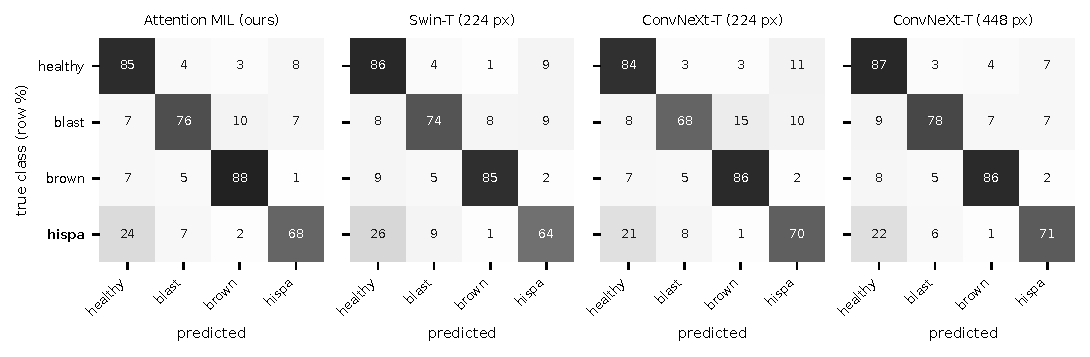
\includegraphics[width=0.8\textwidth]{final_confusion.pdf}
\caption{Row-normalised confusion matrices (\% of the true class) of four methods on the session-blocked test photos, pooled over the 5 rounds. The bold row is hispa, the pre-declared diagnostic class; counts are in Table~\ref{tab:final_confusion}.}
\label{fig:confusion}
\end{figure*}

Table~\ref{tab:final_per-class} gives per-class recall. For every method the lowest-recall class is hispa or leaf blast:
hispa for 8 of the 11 methods, including Attention MIL (67.6\,\%), and leaf blast for InceptionV3, ConvNeXt-T at 224 px and
the same head on whole photos at 512 px. Hispa recall ranges from 57.8 to 73.0\,\% across methods, so the two hardest
classes are the same for every method: a property of the classes, not of one model. Hispa recall was declared in advance
as a diagnostic, because hispa damage (pale scraped streaks) can look like healthy or lightly damaged tissue.
Fig.~\ref{fig:confusion} and Table~\ref{tab:final_confusion} show that this is what happens: 134 of the 564 hispa photos
are called healthy by Attention MIL (381 are correct), and 111 of the 1{,}480 healthy photos are called hispa. The other three
methods in the figure show the same pattern. Leaf-blast photos are spread over all three other classes (Attention MIL: 54
healthy, 77 brown spot, 55 hispa, of 773), and Attention MIL's recall on brown spot (88.0\,\%) is the highest in the table.

\subsection{Zero-shot transfer to field photos (H3)}
\begin{figure}[t]
\centering
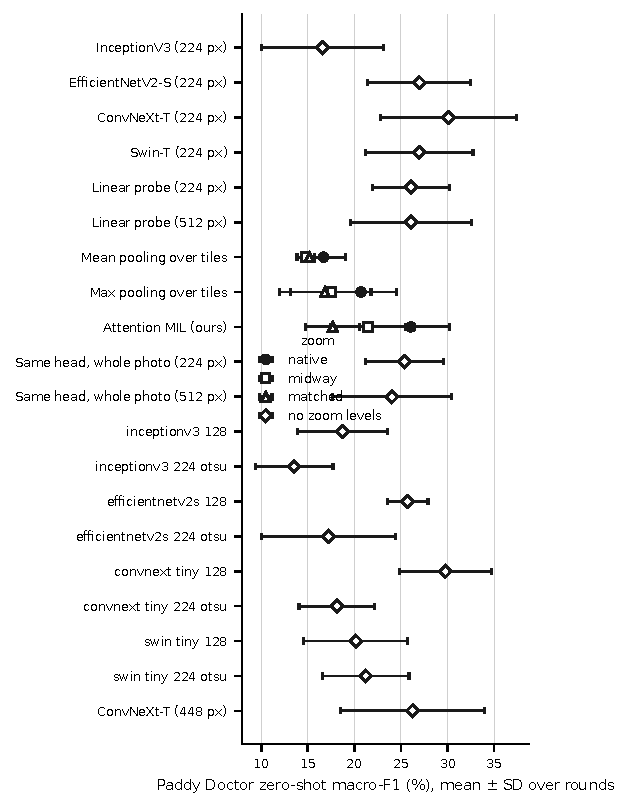
\includegraphics[width=0.8\columnwidth]{final_paddy_zoom.pdf}
\caption{Zero-shot macro-F1 (\%) on Paddy Doctor, mean $\pm$ SD over the 5 round-models, for every method and condition; the tile methods are shown at native, midway and matched zoom.}
\label{fig:paddy-zoom}
\end{figure}

On Paddy Doctor (native zoom, Table~\ref{tab:final_main}) Attention MIL scores 26.1 $\pm$ 4.2 macro-F1 and 33.8 $\pm$ 2.9
balanced accuracy, where 25.0 is chance for balanced accuracy. Every method, including the 128-px and Otsu conditions, falls
between 13.5 and 30.1 macro-F1; ConvNeXt-T at 224 px is highest (30.1 $\pm$ 7.3). By the rule declared before the run, H3 holds if
Attention MIL beats each of the four fine-tuned 224-px models; it beats only InceptionV3 (+13.9), so \textbf{H3 is not
shown}. Pooling the five round-models of each method, EfficientNetV2-S and ConvNeXt-T at 224 px scored higher than Attention MIL
(by 3.8 and 4.3 points; their ranges lie entirely below zero), but the declared rule asks for one direction only and calls
these ``no clear difference''. Many models predict almost one class for every field photo: pooled over its five
round-models, Attention MIL recalls 79.2\,\% of leaf-blast photos but 0.1\,\% of healthy photos. Matching the zoom did not help the tile methods:
Attention MIL scores 21.5 at midway and 17.7 at matched zoom (Table~\ref{tab:final_main}; Fig.~\ref{fig:paddy-zoom}).

\subsection{Do the heat maps point at symptoms (H4)?}
\PaperTable[\SmallWide]{explain}{Deletion test on the session-blocked test photos (seed-0 models): macro-F1 (\%) after removing the $k$ most-attended tiles or $k$ random tiles, and the true-class probability gap (random minus top-$k$ removed, points) with 95\,\% photo and block ranges and rounds won.}

\PaperTable[\SmallWide]{explain_ratings}{Blind ratings of 50 heat maps (validation photos) by two independent sets of three model raters: share of each answer to ``does the hot area cover visible symptoms?'', share of maps on which all three raters agree, and Fleiss' $\kappa$.}

\begin{figure*}[t]
\centering
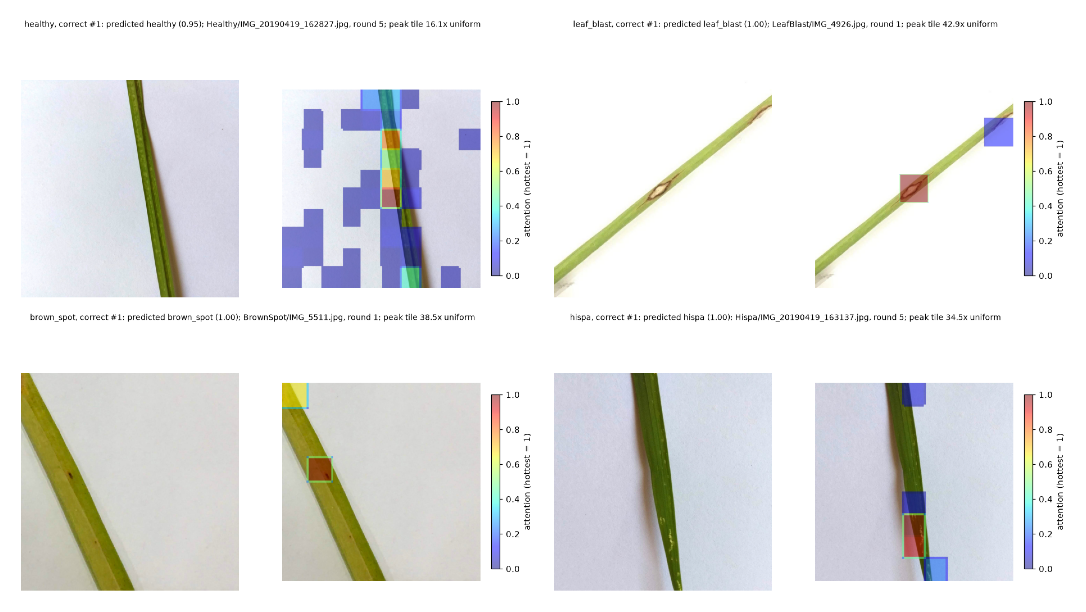
\includegraphics[width=0.7\textwidth]{final_heatmaps.pdf}
\caption{Heat maps for the most confident correct validation photo of each class (photo and attention overlay). These are the best case of each class, not typical examples; colour is attention relative to the photo's maximum and not a disease probability.}
\label{fig:heatmaps}
\end{figure*}

In the deletion test, in the spirit of RISE \cite{petsiuk2018rise}, we removed the $k$ most-attended tiles or $k$ random tiles from each test photo and rescored it
(Table~\ref{tab:final_explain}). Removing 16 attended tiles lowers macro-F1 from 77.9 to 15.6, while removing 16 random
tiles lowers it only to 75.3. The true-class probability falls 25.4 points more after the attended tiles are removed
(photo range $[24.5, 26.2]$, block range $[18.2, 32.8]$, 5 of 5 rounds), and the gap grows with $k$. It is negative for
healthy photos ($-12.9$ at $k=16$), which have no symptom to find. On Paddy Doctor photos the effect is small (2.2 points
at $k=16$, photo range only). On the test photos Attention MIL puts 15.3\,\% of its attention on background tiles, which are
74.5\,\% of all tiles; on Paddy Doctor photos attention on background (20.3\,\%) is no different from the tile share (19.7\,\%).
Two independent sets of three disclosed model raters rated 50 blind heat maps of validation photos
(Fig.~\ref{fig:heatmaps}, Table~\ref{tab:final_explain-ratings}): the hot area covers visible symptoms for 39.3\,\% (set 1)
and 49.3\,\% (set 2) of the ratings, partly for 32.0 and 24.0\,\%, and not for 28.7 and 26.7\,\%. Fleiss' $\kappa$
\cite{fleiss1971kappa} is 0.88 and 0.75, and the majority answers of the two sets agree on 84.0\,\% of the maps. The
heat maps are qualitative evidence of where the head looks; they carry no severity claim.

\subsection{Cost (H5)}
\PaperTable[\WideLayout]{cost}{Parameters (M), disk size (MB), training cache (GB), time per photo (s) on GPU and CPU, peak GPU and CPU memory (MB) and test macro-F1 (\%). Times are medians over 100 photos, one at a time from disk, decoding included, on one machine (RTX 4060, Ryzen 7 7700) and depend on it.}

\begin{figure}[t]
\centering
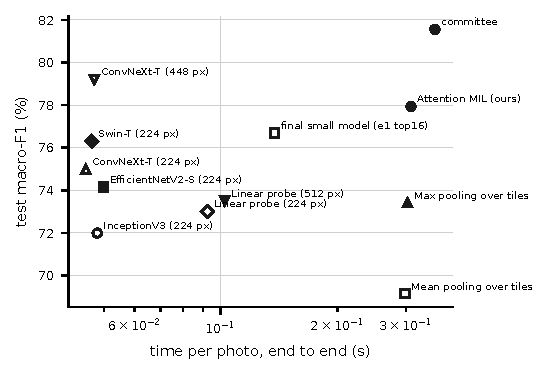
\includegraphics[width=\columnwidth]{final_cost.pdf}
\caption{Test macro-F1 (\%) against time per photo, end to end (log scale), session-blocked split; one machine (RTX 4060 GPU).}
\label{fig:cost}
\end{figure}

Table~\ref{tab:final_cost} and Fig.~\ref{fig:cost} give the cost. Attention MIL needs about 79 encoder passes per photo, so it takes 0.31 s per
photo on the GPU and 5.36 s on the CPU, about 80 times the 224-px whole-image models on the CPU (0.06--0.07 s); the head is small, but the frozen encoder must run for every tile. Compression variants were scored on validation photos
(reference 78.5, 5.36 s on the CPU): keeping 16 tiles gave 76.5 at 1.21 s; a head distilled from the smaller DINOv3
ViT-S/16 gave 78.6; 8-bit linear layers failed (23.6); and the 16-tile model exported to ONNX took 0.93 s on the CPU. The
Small model (16 tiles) was tested once and scores 76.7 on test, with no clear difference from Attention MIL ($+1.4$, 3 of 5
rounds). No rule for H5 was declared, so this is a descriptive answer; times are from one machine and depend on its hardware.

\subsection{Partition order}
\begin{figure}[t]
\centering
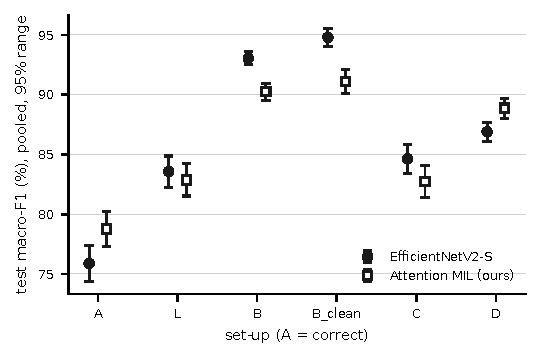
\includegraphics[width=\columnwidth]{final_partition_order.pdf}
\caption{Partition-order experiment: pooled test macro-F1 (\%) with 95\,\% ranges. A: session-blocked split, augmentation on training photos only (correct); L: locked split; B: augment first, then split the copies at random; B\_clean: B scored on clean copies only; C: random split without grouping; D: train and score on the same photos. Full table in Table~\ref{tab:final_partition-order}.}
\label{fig:partition-order}
\end{figure}

Fig.~\ref{fig:partition-order} shows how much three faulty set-ups raise the score of two models trained under the
correct protocol (A). The set-ups are deliberately wrong and are not estimates of performance. Augmenting every photo eight
times and then splitting the copies at random (B) raises macro-F1 by 17.2 points for EfficientNetV2-S and 11.5 for Attention MIL
(pooled scores, both clearly above A). Splitting photos at random without grouping (C) raises it by 8.8 and 4.0, and
training and scoring on the same photos (D) by 11.0 and 10.1. The locked split (L) is 7.7 and 4.1 points above A. The
pattern holds for both models, so the order of splitting and augmenting changes a score by more than most differences
between methods in this field.

\section{Discussion}
\label{sec:discussion}

This section interprets the results against the five hypotheses and the seven objectives; the numbers are in
Section~\ref{sec:results}.

\textbf{H1, tiles against whole-photo input: supported on the headline split.} With the same encoder and head, tiles at
a common leaf scale beat one whole-photo description at both sizes. Two further observations point the same way:
whole-image scores rise with input size (Table~\ref{tab:final_conditions}), and tiles at the stored scale do worse than
tiles at the common scale (Table~\ref{tab:final_ablations-test}). Detail matters. It does not follow that tiling matters:
ConvNeXt-T at 448 px has the higher mean and the paired test finds no clear difference. What the tile pipeline offers is a
different cost profile, a small head trained from cached descriptions, against fine-tuning a whole network at
a larger input size. The Committee gain suggests that the two kinds of model make partly different errors.
On the locked split the benefit over the 512-px control was not clear, which is a reminder that the split changes
conclusions.

\textbf{H2, attention against mean, max and Otsu: supported.} Most tiles hold background, and the head gives them far less than their share of its attention (Section~\ref{sec:results}). Mean pooling averages all of them with the few informative
tiles, which is a likely reason for its low score; max pooling keeps the single strongest tile and comes close, without a clear
difference on balanced accuracy. Hard background removal by Otsu's method did not help whole-image models and lowered the
tile model, so a learned weighting looked more useful than a fixed mask; an earlier report found Otsu alone changed
accuracy little \cite{ali2026}.

\textbf{H3, frozen features on field photos: not shown.} All methods score low on Paddy Doctor and none is clearly
ahead of the fine-tuned models, so in-domain scores say little about field behaviour. Matching the zoom did not
help. We did not test the likely causes, such as lighting, camera and field context, and the primary photos have plain
backgrounds (Section~\ref{sec:setup:data}); we therefore do \emph{not} claim robustness to clutter.

\textbf{H4, heat maps point at symptoms: supported as a qualitative guide.} The deletion test shows that the decision
rests on the attended tiles, but that alone does not show that those tiles are symptoms. The ratings are mixed, and about a
quarter of the ratings in each set say no. The effect on field photos is small. We treat heat maps as an aid for a reader,
not as a segmentation, and make no severity claim.

\textbf{H5, cost: a descriptive answer.} The pipeline is slower per photo than whole-image models because of its many
encoder passes. Fewer tiles and a distilled head reduce the cost at little loss of validation score, but the 8-bit encoder
fails, so an on-device build is not shown.

\textbf{What the shortcut and split checks mean for reading in-domain numbers.} The nearest-in-time baseline matches
the models on the locked split, and the partition-order experiment shows that the order of augmenting and splitting
moves a score more than most differences between methods. We therefore read differences between methods only on the
session-blocked split and only through the paired rule, and we state the split beside every number. This is a general
lesson for the field rather than a verdict on any study: the details of splitting are rarely reported
\cite{xu2024}. The per-class results add that hispa and leaf blast are hard for every method, so a single accuracy figure
hides the classes where errors concentrate; hispa photos are most often called healthy.

\textbf{Objectives.} Table~\ref{tab:objectives} relates the seven objectives to the evidence.

\begin{table}[t]
\caption{The seven objectives, the evidence and the status.}
\label{tab:objectives}
\centering
\scriptsize
\renewcommand{\arraystretch}{1.1}
\begin{tabular}{@{}L{3.1cm}L{3.5cm}L{1.1cm}@{}}
\toprule
Objective & Evidence & Status \\
\midrule
1 Two-dataset benchmark & Primary photos and Paddy Doctor (Section~\ref{sec:setup:data}) & met \\
2 Leakage-free protocol & Grouped splits made first, mean $\pm$ SD, two ranges, one rule (Section~\ref{sec:setup}) & met \\
3 Whole-image baselines, including Otsu & Four models at 128, 224 and 448 px, with and without Otsu (Tables~\ref{tab:final_main}, \ref{tab:final_conditions}) & met \\
4 Tile-based weakly supervised model & Attention MIL (Section~\ref{sec:method}) & met \\
5 Ablations of resolution, aggregation, Otsu & Tables~\ref{tab:final_conditions}, \ref{tab:final_main}, \ref{tab:final_ablations-test}, \ref{tab:final_ablations} & met \\
6 Zero-shot transfer; attention against symptoms & Paddy Doctor (H3 not shown); deletion test and model-rater ratings; no expert or outline check & partly met \\
7 Cost and compressibility & Table~\ref{tab:final_cost}; fewer tiles and distillation help, 8-bit fails; no on-device build & partly met \\
\bottomrule
\end{tabular}
\end{table}

\section{Limitations and Future Work}
\label{sec:limits}

Table~\ref{tab:limits} pairs each limitation with the finding it rests on and the next step that builds on it.

\begin{table}[t]
\caption{Limitations, the findings they rest on, and the next steps.}
\label{tab:limits}
\centering
\scriptsize
\renewcommand{\arraystretch}{1.1}
\begin{tabular}{@{}L{2.3cm}L{2.2cm}L{3.3cm}@{}}
\toprule
Limitation & Finding & Next step \\
\midrule
The encoder is frozen and never adapted to rice; field transfer fails & H3 not shown (Section~\ref{sec:res:paddy}) & Light fine-tuning of the encoder; open-set handling and adaptation using the other nine Paddy Doctor classes \\
About 79 encoder passes per photo; timing from one machine & Cost, small model, 8-bit failure (Section~\ref{sec:res:cost}) & An on-device build, timed on more than one device \\
Heat maps are qualitative; no severity labels & Deletion test and ratings of 50 maps (Section~\ref{sec:res:explain}) & Check attention against lesion outlines (RiceSeg-5932 \cite{riceseg2025}); a rating study with plant-disease experts \\
One region, one set of cameras, four classes, no bacterial leaf blight & Setup (Section~\ref{sec:setup:data}) & Dhan-Shomadhan \cite{hossain2021} as a further test set; bacterial leaf blight from Paddy Doctor \\
Labels may hold noise; plain backgrounds & Background audit and label check (Section~\ref{sec:setup:data}) & Data with cluttered backgrounds and severity scores \\
The leaf-scale rule is borderline; zero-shot scores depend on the zoom & Leaf-width audit (Section~\ref{sec:setup:data}), zoom levels & More leaf-width measurements \\
One training seed per round (compute limits); some comparisons were declared after the means were seen & Sections~\ref{sec:setup:metrics}, \ref{sec:results} & Several seeds per round; declare the committee and 448-px tests in advance on new photos \\
\bottomrule
\end{tabular}
\end{table}

\section{Conclusion}
\label{sec:conclusion}

We treated image resolution as a variable and the evaluation protocol as part of the method. A frozen DINOv3 encoder, high-detail
tiles at a common leaf scale and a small attention head trained from photo labels gave a rice leaf disease classifier
with a heat map. Under a protocol that groups near-duplicates and capture sessions, it was clearly better than
whole-photo use of the same encoder and than simpler pooling, and not clearly different from a ConvNeXt-T fine-tuned at a larger input size; combining
the two kinds of model helped. It did not transfer to field photos, and its price is many encoder passes per photo. The
partition-order experiment and the controls that never see the leaf show that the split, not only the model, decides how
good a score looks. Much published work reports a single downsampled view and leaves the split order unstated; stating
both, with paired rules and negative results, is what we offer as a basis for future comparisons.


\appendices
\section{Secondary Results and Settings}
\label{sec:appendix}

This appendix holds the secondary tables cited in the text. The training settings are in Section~\ref{sec:setup:training}.

\PaperTable[\SmallWide]{ablations}{All ablations on validation photos: macro-F1 (\%), mean $\pm$ SD over the 5 rounds, session-blocked split. Validation scores favour the main configuration (Attention MIL), whose settings were chosen on them; the variants were not tuned.}

\PaperTable[\SmallWide]{paired_conditions}{Attention MIL against each whole-image condition at 128 px and with Otsu, session-blocked test photos: difference of the pooled scores in points (Attention MIL minus the condition), 95\,\% ranges, rounds won, and verdicts. Declared after the means were seen.}

\PaperTable[\SmallWide]{paired_locked}{Attention MIL against every whole-image model and control on the locked split, test photos: difference of the pooled scores in points (Attention MIL minus the other), 95\,\% ranges, rounds won, and verdicts.}

\PaperTable[\SmallWide]{confusion}{Confusion matrices (photo counts) of four methods on the session-blocked test photos, pooled over the 5 rounds. Rows are the true class.}

\PaperTable[\SmallWide]{partition_order}{Partition-order experiment: pooled macro-F1 (\%) and its inflation over the correct set-up (A), with 95\,\% ranges, for EfficientNetV2-S and Attention MIL. L is the locked split; B, C and D are deliberately faulty set-ups (augment first, then split the copies at random; random split without grouping; train and score on the same photos) and are not estimates of performance.}



\clearpage

\section*{Acknowledgements}
{\raggedright
This work uses DINOv3 \cite{simeoni2025dinov3}, which is
distributed under the DINOv3 License; as the licence requires, we acknowledge its use. The model versions
are \path{facebook/dinov3-vitb16-pretrain-lvd1689m} (revision \path{5931719e}) and
\path{facebook/dinov3-vits16-pretrain-lvd1689m} (revision \path{114c1379}). The primary dataset is
released under the MIT licence \cite{do2019} and Paddy Doctor under CC~BY~4.0 \cite{petchiammal2023}.\par}

\printbibliography

\end{document}
